% RistrettoPoint.conditional_select_spec: dependency closure and the
% agent's bottom-up proof (run topspec_2026-09-24T084820+0000, accepted).
% Page 1: dependency graph.  Page 2: proof timeline.
% Build: pdflatex ristretto_conditional_select.tex
%        pdftoppm -png -r 300 ristretto_conditional_select.pdf ristretto_cs
\documentclass[tikz,border=8pt]{standalone}
\usepackage[T1]{fontenc}
\usepackage{lmodern}
\renewcommand{\familydefault}{\sfdefault}
\usetikzlibrary{positioning,arrows.meta,fit,backgrounds,calc}

\definecolor{given}{RGB}{225,225,225}
\definecolor{givenline}{RGB}{140,140,140}
\definecolor{agent}{RGB}{214,240,214}
\definecolor{agentline}{RGB}{60,140,60}
\definecolor{top}{RGB}{210,225,250}
\definecolor{topline}{RGB}{50,90,170}
\definecolor{fail}{RGB}{250,215,210}
\definecolor{failline}{RGB}{190,60,50}

\tikzset{
  box/.style={draw, rounded corners=3pt, line width=0.9pt, align=center,
              minimum width=6.4cm, minimum height=1.25cm, inner sep=5pt},
  givenbox/.style={box, fill=given, draw=givenline},
  agentbox/.style={box, fill=agent, draw=agentline},
  topbox/.style={box, fill=top, draw=topline},
  call/.style={-{Stealth[length=3mm]}, line width=1pt},
  note/.style={font=\small, align=left, text width=5.6cm},
  lab/.style={font=\small\itshape, fill=white, inner sep=2pt},
}

\begin{document}

%% ---------------------------------------------------------------- page 1
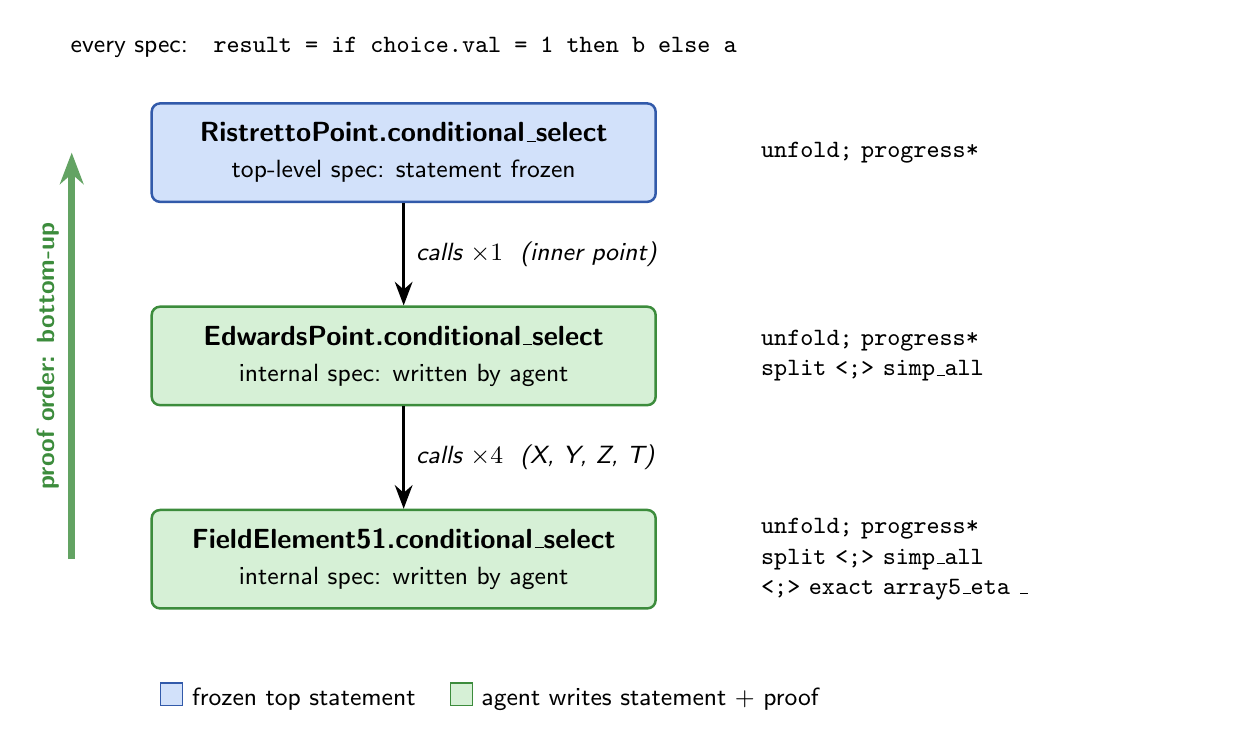
\begin{tikzpicture}[node distance=1.3cm]
  \node[topbox] (ris) {\textbf{RistrettoPoint.conditional\_select}\\[1pt]
    \small top-level spec: statement frozen};
  \node[agentbox, below=of ris] (ed) {\textbf{EdwardsPoint.conditional\_select}\\[1pt]
    \small internal spec: written by agent};
  \node[agentbox, below=of ed] (fe) {\textbf{FieldElement51.conditional\_select}\\[1pt]
    \small internal spec: written by agent};

  \draw[call] (ris) -- node[lab, right=2pt] {calls $\times 1$ \ (inner point)} (ed);
  \draw[call] (ed)  -- node[lab, right=2pt] {calls $\times 4$ \ (X, Y, Z, T)} (fe);

  % proof per level
  \node[note, right=1.2cm of ris] {\texttt{unfold; progress*}};
  \node[note, right=1.2cm of ed]  {\texttt{unfold; progress*}\\\texttt{split <;> simp\_all}};
  \node[note, right=1.2cm of fe]  {\texttt{unfold; progress*}\\\texttt{split <;> simp\_all}\\
                                   \texttt{<;> exact array5\_eta \_}};

  % same statement shape for all three
  \node[font=\small, align=center, above=0.45cm of ris] {every spec:\quad
    \texttt{result = if choice.val = 1 then b else a}};

  % proof order arrow
  \coordinate (b) at ($(fe.west)+(-1.0cm,0)$);
  \coordinate (t) at ($(ris.west)+(-1.0cm,0)$);
  \draw[-{Stealth[length=4mm]}, line width=2.5pt, agentline!80] (b) --
    node[sloped, above, font=\small\bfseries, text=agentline] {proof order: bottom-up} (t);

  % legend
  \node[below=0.8cm of fe.south west, anchor=north west, font=\small] (lg) {%
    \tikz\node[fill=top,draw=topline,minimum size=8pt]{}; frozen top statement \quad
    \tikz\node[fill=agent,draw=agentline,minimum size=8pt]{}; agent writes statement + proof};
\end{tikzpicture}

%% ---------------------------------------------------------------- page 2
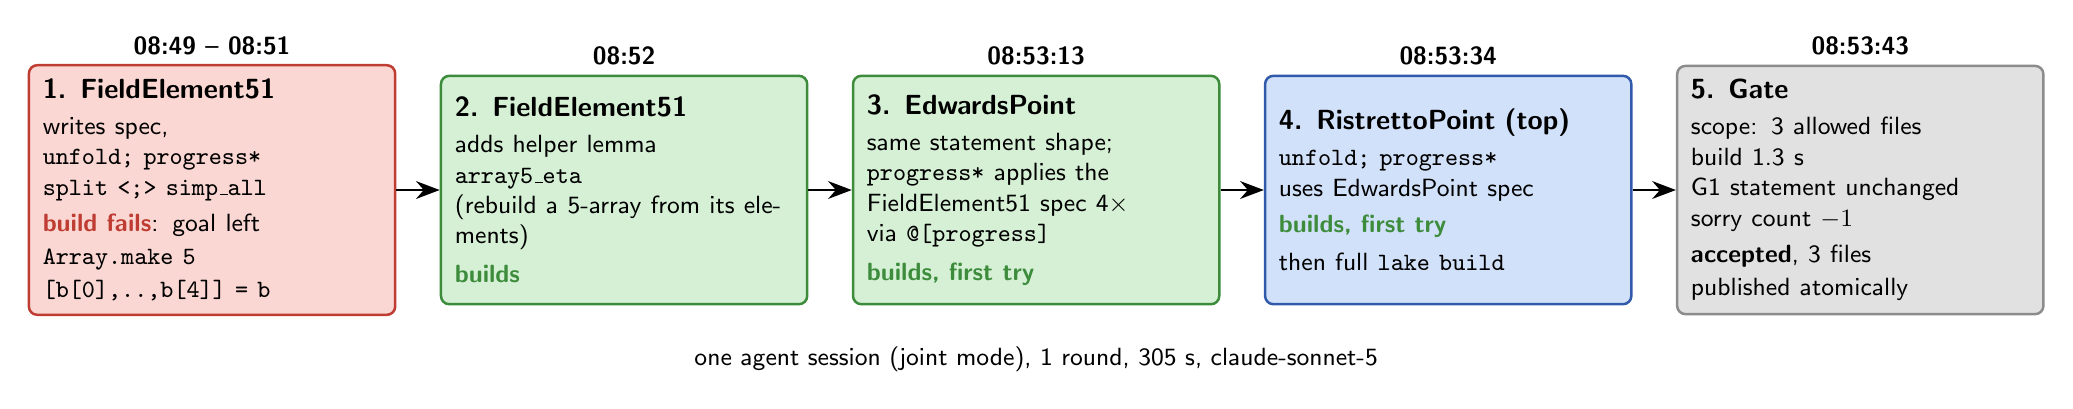
\begin{tikzpicture}[
    stepbox/.style={box, minimum width=4.6cm, minimum height=2.9cm, text width=4.3cm, align=left},
    t/.style={font=\small\bfseries, anchor=south},
    node distance=0.55cm]

  \node[stepbox, fill=fail, draw=failline] (s1) {%
    \textbf{1. FieldElement51}\\[2pt]
    \small writes spec,\\ \texttt{unfold; progress*}\\\texttt{split <;> simp\_all}\\[2pt]
    \textcolor{failline}{\textbf{build fails}}: goal left\\
    \texttt{Array.make 5 [b[0],..,b[4]] = b}};
  \node[stepbox, fill=agent, draw=agentline, right=of s1] (s2) {%
    \textbf{2. FieldElement51}\\[2pt]
    \small adds helper lemma\\ \texttt{array5\_eta}\\
    (rebuild a 5-array from its elements)\\[2pt]
    \textcolor{agentline}{\textbf{builds}}};
  \node[stepbox, fill=agent, draw=agentline, right=of s2] (s3) {%
    \textbf{3. EdwardsPoint}\\[2pt]
    \small same statement shape;\\ \texttt{progress*} applies the\\
    FieldElement51 spec 4$\times$\\ via \texttt{@[progress]}\\[2pt]
    \textcolor{agentline}{\textbf{builds, first try}}};
  \node[stepbox, fill=top, draw=topline, right=of s3] (s4) {%
    \textbf{4. RistrettoPoint (top)}\\[2pt]
    \small \texttt{unfold; progress*}\\ uses EdwardsPoint spec\\[2pt]
    \textcolor{agentline}{\textbf{builds, first try}}\\[2pt]
    then full \texttt{lake build}};
  \node[stepbox, fill=given, draw=givenline, right=of s4] (s5) {%
    \textbf{5. Gate}\\[2pt]
    \small scope: 3 allowed files\\ build 1.3 s\\ G1 statement unchanged\\
    sorry count $-1$\\[2pt]
    \textbf{accepted}, 3 files\\ published atomically};

  \foreach \a/\b in {s1/s2, s2/s3, s3/s4, s4/s5}
    \draw[call] (\a) -- (\b);

  \node[t] at (s1.north) {08:49 -- 08:51};
  \node[t] at (s2.north) {08:52};
  \node[t] at (s3.north) {08:53:13};
  \node[t] at (s4.north) {08:53:34};
  \node[t] at (s5.north) {08:53:43};

  \node[font=\small, below=0.4cm of s3] {one agent session (joint mode), 1 round, 305 s,
    claude-sonnet-5};
\end{tikzpicture}

\end{document}
